\begingroup
\newcommand{\SevenCoil}{
\draw (0,0)
foreach \i in {1,...,7}{
.. controls ({.42*\i-.37},.25) and ({.42*\i},.25) .. ({.42*\i},0)
.. controls ({.42*\i},-.16) and ({.42*\i-.13},-.16) .. ({.42*\i-.13},0)
}
.. controls (2.81,.25) and (3.36,.25) .. (3.36,0);
}
\begin{center}
\begin{tikzpicture}[x=.85cm,y=.85cm,line width=.55pt]
\begin{scope}[shift={(0,3.4)}]\SevenCoil\end{scope}
\draw (0,3.4)--(0,1.6).. controls (0,.55) and (.5,0) .. (1.65,0)
.. controls (2.8,0) and (3.36,.55) .. (3.36,1.6)--(3.36,3.4);
\draw (1.65,0) circle[radius=.25];
\draw[->,>=stealth] (1.15,-.52)--(2.17,.56);
\node[above] at (1.68,3.53) {$e(r)$};\node[below right,inner sep=1pt] at (1.9,-.10) {$M(1)$};
\node[below] at (1.68,-.85) {$a=\dfrac{e}{1+r}$};
\begin{scope}[shift={(5.3,0)}]
\begin{scope}[shift={(0,3.4)}]\SevenCoil\end{scope}
\draw (0,3.4)
foreach \i in {1,...,8}{
.. controls (-.27,{3.4-.38*\i+.33}) and (-.27,{3.4-.38*\i}) .. (0,{3.4-.38*\i})
.. controls (.17,{3.4-.38*\i}) and (.17,{3.4-.38*\i+.13}) .. (0,{3.4-.38*\i+.13})
}
.. controls (-.27,.49) and (-.27,0) .. (0,0)--(1.65,0)
.. controls (2.8,0) and (3.36,.55) .. (3.36,1.6)--(3.36,3.4);
\draw (1.65,0) circle[radius=.25];
\draw[->,>=stealth] (1.15,-.52)--(2.17,.56);
\node[above] at (1.68,3.53) {$e(r)$};\node[right,inner sep=1pt] at (.26,1.8) {$E(R)$};
\node[below right,inner sep=1pt] at (1.9,-.10) {$M(1)$};
\node[below] at (1.68,-.85) {$b=\dfrac{e}{1+r+R}$};
\end{scope}
\begin{scope}[shift={(10.6,0)}]
\begin{scope}[shift={(0,3.4)}]\SevenCoil\end{scope}
\draw (0,3.4)--(0,1.6).. controls (0,.55) and (.5,0) .. (1.65,0)
.. controls (2.8,0) and (3.36,.55) .. (3.36,1.6)--(3.36,3.4);
\begin{scope}[shift={(0,1.8)}]\SevenCoil\end{scope}
\draw (1.65,0) circle[radius=.25];
\draw[->,>=stealth] (1.15,-.52)--(2.17,.56);
\node[above] at (1.68,3.53) {$e(r)$};\node[above] at (1.68,1.95) {$E(R)$};
\node[below right,inner sep=1pt] at (1.9,-.10) {$M(1)$};
\node[below] at (1.68,-.85) {$c=\dfrac{eR}{r+R+rR}$};
\end{scope}
\end{tikzpicture}
\end{center}
\endgroup
